% 玻尔原子模型
% 玻尔|原子|半经典|氢原子|类氢原子

\pentry{圆周运动\upref{CMAD}, 库仑力\upref{ClbFrc}}

\begin{figure}[ht]
\centering
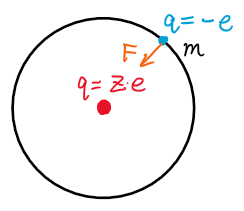
\includegraphics[width=4cm]{./figures/BohrMd1.png}
\caption{玻尔原子模型} \label{BohrMd_fig1}
\end{figure}

\textbf{玻尔原子模型(Bohr Model)}(\autoref{BohrMd_fig1})是量子力学发展的早期被提出的一种解释\textbf{类氢原子}光谱的模型. 该模型中, 我们假设原子核具有 $Z$ 个正电荷。 对于氢原子 $H$ 有 $Z = 1$, 氦离子 $He^+$ 有 $Z = 2$, 锂离子 $Li^{++}$ 有 $Z = 3$ 等等。

由于原子核质量远大于电子, 我们先假设它固定不动, % 未完成: 约化玻尔模型
唯一的核外电子按照牛顿力学和库伦定律运动, 再人为地加上一个条件(\textbf{量子化条件})使电子的轨道角动量只能取一些特定的(\textbf{离散}的)值. 这样, 轨道的半径也只能取离散的值, 每个半径 $r_n$ 对应一个机械能(动能加势能) $E_n$, 我们把这些能量叫做\textbf{能级}. 如果电子从一条能量较高的轨道跃迁到另一条能量较低的轨道, 那么一个光子将被产生, 带走两个轨道的能量差. 反之, 如果恰好有一个入射光子的能量是两条轨道机械能之差, 那这个光子就可以被低能量轨道的电子吸收, 使其跃迁到高能量轨道.

虽然这个模型成功地解释了氢原子各个能级的能量以及氢原子光谱%未完成, 介绍一下
, 但它却并不是完全按照量子力学的的方法来计算的. 按照(现代的)量子力学, 电子需要用波函数描述, 波函数由薛定谔方程计算得到, 所以不具有经典力学中“轨道” 的概念.

根据玻尔模型, 氢原子的各个能级的能量为
\begin{equation}
E_n =  - \frac{m e^4}{32 \pi^2 \epsilon_0^2 \hbar ^2} \frac{Z^2}{n^2} \approx - 13.6\Si{eV} \frac{Z^2}{n^2}
\qquad (n = 1, 2, \dots)
\end{equation}
可见 $n$ 越大, 能级越高. 我们把 $n = 1$ 的状态叫做\textbf{基态}, 其他状态叫做\textbf{激发态}. 

各能级的轨道半径如下. 特殊地, 我们把氢原子基态($Z = 1$, $n = 1$) 的电子轨道的半径叫做\textbf{玻尔半径}, 记为 $a_0$.
\begin{equation}\label{BohrMd_eq1}
r_n = a_0 \frac{n^2}{Z}
\qquad (n = 1, 2, \dots)
\end{equation}
\begin{equation}
a_0 = \frac{4\pi \epsilon_0 \hbar^2}{m e^2} \approx 5.292\times 10^{-11}\Si{m}
\end{equation}


\subsection{能级公式推导}
% 未完成, 应该给出 $r_n$ 的公式
所有原子中最简单的一类叫\textbf{类氢原子},类氢原子只有一个核外电子,以及一个带 $Z$ 个元电荷的原子核.以下的计算假设二者为质点和点电荷,原子核不动,电子绕原子核做圆周运动.运用经典力学和库仑力公式,可求出电子在不同半径下做圆周运动的能量. 库仑定律与牛顿定律(圆周运动)分别为
\begin{equation}
F = \frac{1}{4\pi \epsilon_0} \frac{(Ze)e}{r^2}
\qquad
F = ma = m\frac{v^2}{r}
\end{equation}
解得电子速度平方为
\begin{equation}\label{BohrMd_eq2}
v^2 = \frac{e^2 Z}{4\pi \epsilon_0 mr}
\end{equation}
动能与势能分别为
\begin{equation}
E_K = \frac12 m v^2 = \frac{1}{8\pi\epsilon_0} \frac{Z e^2}{r}
\qquad
E_P =  -\frac{1}{4\pi\epsilon_0} \frac{Ze^2}{r} = -2 E_k
\end{equation}   
总能量为
\begin{equation}\label{BohrMd_eq4}
E = E_K + E_P =  -\frac{Z e^2}{8\pi\epsilon_0 r}
\end{equation}
到此为止,我们还没有用到量子力学.然而这样的模型与真实的类氢原子相比有两个致命的缺陷: 第一,根据电动力学,圆周运动的电子会向外辐射电磁波,能量减少,最终坠入原子核; 第二,该模型允许氢原子的能量具有连续值(因为 $r$ 可连续变化),而实验中氢原子只能放出特定能量的光子,说明只能取特定的能量,即存在离散的\textbf{能级},我们把能级由低到高记为 $E$  $(n = 1,2,3\dots)$. 

以上矛盾说明微观世界的粒子不遵守经典力学和电磁学.玻尔为了解释实验,在经典力学和电磁学上加入了一个条件: 角动量量子化.

以原子核为原点,电子轨道平面的法向量为 $z$ 轴,由于电子的位矢 $\bvec r$ 与动量 $\bvec p$ 始终垂直,电子的角动量为
\begin{equation}
\bvec L = \bvec r \cross \bvec p = mvr \uvec z
\end{equation}
玻尔引入的角动量量子化条件为
\begin{equation}\label{BohrMd_eq6}
L = mvr = n\hbar
\end{equation}
其中 $n$ 可以取任意正整数, $\hbar$ 为\textbf{约化普朗克常量}
\begin{equation}\label{BohrMd_eq7}
\hbar  = \frac{h}{2\pi}
\end{equation}
该条件也可以等效理解为驻波条件,即允许的圆形轨道长度是德布罗意波% 在量子力学基本假设中提一下德布罗意波长, 未完成,引用
长的整数倍.
\begin{equation}\label{BohrMd_eq8}
2\pi r  = \frac{h}{mv} n
\end{equation}
注意\autoref{BohrMd_eq6} 与\autoref{BohrMd_eq8} 等效.把\autoref{BohrMd_eq2} 带入了该条件,解得可能的轨道半径为\autoref{BohrMd_eq1}. 注意轨道与 $n^2$ 成正比, 和 $Z$ 成反比.

将 $r_n$(\autoref{BohrMd_eq1}) 代入\autoref{BohrMd_eq4}, 得到能级表达式为
\begin{equation}\label{BohrMd_eq11}
E_n =  - \frac{mZ^2 e^4}{32\pi^2\epsilon_0^2 \hbar ^2} \frac{1}{n^2} \approx  - 13.6\Si{eV}\frac{Z^2}{n^2}
\end{equation}
对氢原子, 有 $Z = 1$, 最低的能级为 $n = 1$, 所以氢原子\textbf{基态}的能级 $E_0$ 约为 $-13.6\Si{eV}$. 这是一个著名的常数(若使用原子单位\upref{AU}, 这个值恰好是 $-1/2$).

将 $r_n$ 带入\autoref{BohrMd_eq2} 还可以得到电子速度为
\begin{equation}\label{BohrMd_eq10}
v_n = \frac{Z e^2}{4\pi\epsilon_0\hbar} \frac{1}{n}
\end{equation}
